\documentclass[11pt,a4paper]{article}
\usepackage[a4paper, margin=1.3in]{geometry}
\usepackage{mathtools}
\usepackage{graphicx}
\usepackage{fancyhdr}
\pagestyle{fancy}
\usepackage{lastpage}

\usepackage {tikz}
\usetikzlibrary {positioning}
%\usepackage {xcolor}
\definecolor {processblue}{cmyk}{0.96,0,0,0}

\fancyhf{}
\lhead{AI Planning}
\rhead{Exercise Sheet 4}
\lfoot{Axel Perschmann, Tarek Saier, 20.11.2014}
\rfoot{Page \thepage\ of \pageref{LastPage}}
\renewcommand{\headrulewidth}{0.3pt}
\renewcommand{\footrulewidth}{0.3pt}
\setlength\parindent{0pt}

\begin{document}
\begin{center}
\Huge{\textbf{AI Planning}}\\
\LARGE{\textbf{Exercise Sheet 4}}
\end{center}
\vspace{2cm}
\begin{tabular}{ll}
Date: & 20.11.2014\\
Students: & Axel Perschmann, Tarek Saier
\end{tabular}

\section*{Exercise 4.1}
For easy readability let the tiles be referred to as $b_1$, $b_2$, $w_1$ and $w_2$ and the empty cell be referred to as $e$. Furthermore, let the actions move and jump be denoted as $m_c(t)$ and $j_c(t)$ respectively where $c$ is the destination cell$\in \{1,2,3,4,5\}$ and $t$ is the tile that is being relocated.\\
As an example, the initial state is:\\
$b_1,b_2,w_1,w_2,e$\\
If we then apply $j_5(b_2)$ we reach:\\
$b_1,e,w_1,w_2,b_2$\\
\\
\textbf{(a)} Let $\lceil o\rceil$ denote the state $s$ reached by applying the operation $o\in \{m_c(t),j_c(t)\}$.\\
$f(\lceil m_5(w_2)\rceil)=1+4=5$\\
$f(\lceil j_5(w_1)\rceil)=1+4=5$\\
$f(\lceil j_5(b_2)\rceil)=2+2=4$\\
Apply $j_5(b_2)$ which results in $s_1$:\\
$b_1,e,w_1,w_2,b_2$\\
$f(\lceil m_2(b_1)\rceil)=3+2=5$\\
$f(\lceil m_2(w_1)\rceil)=3+2=5$\\
$f(\lceil j_2(w_2)\rceil)=3+2=5$\\
$\lceil j_2(b_2)\rceil=I\in closed$\\
Apply $m_2(b_1)$ which results in $s_2$:\\
$e,b_1,w_1,w_2,b_2$\\
Apply $m_2(w_1)$ which results in $s_3$:\\
$b_1,w_1,e,w_2,b_2$\\
Apply $j_2(w_2)$ which results in $s_4$:\\
$b_1,w_2,w_1,e,b_2$\\
Expanding on $s_2$:\\
$\lceil m_1(b_1)\rceil=s_1\in closed$\\
$f(\lceil j_1(w_1)\rceil)=4+1=5$\\
$f(\lceil j_1(w_2)\rceil)=5+1=6$\\
Expanding on $s_3$:\\
$f(\lceil j_3(b_1)\rceil)=4+1=5$\\
$f(\lceil m_3(w_1)\rceil)=4+2=6$\\
$f(\lceil m_3(w_2)\rceil)=4+2=6$\\
$f(\lceil j_3(b_2)\rceil)=4+3=7$\\
\\
Expanding on $s_4$:\\
$f(\lceil j_4(b_1)\rceil)=5+0=5$\\
\\
Since $h$ is goal aware and the minimum cost of an operator is 1 we're done at this point. There may be other solutions but none with a cost of less than 5. The resulting plan is: $j_5(b_2),j_2(w_2),j_4(b_1)$ with a total cost of 5 and a final state:\\
$e,w_2,w_1,b_1,b_2$\\

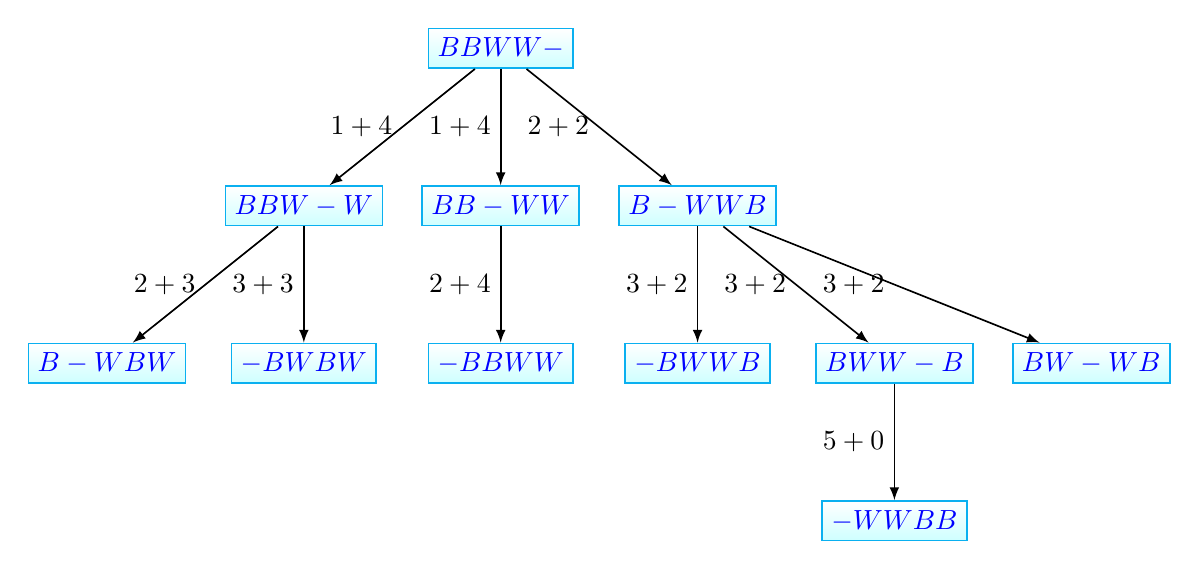
\begin{tikzpicture}[-latex ,auto ,node distance =2 cm and 2.5cm ,on grid ,
semithick ,
state/.style ={top color =white , bottom color = processblue!20 ,
draw,processblue , text=blue }]
\node[state] (A)
{$BBWW-$};
\node[state] (B1) [below left=of A] {$BBW-W$};
\node[state] (B2) [right =of B1] {$BB-WW$};
\node[state] (B3) [right =of B2] {$B-WWB$};
\path (A) edge node[left] {$1+4$} (B1);
\path (A) edge node[left] {$1+4$} (B2);
\path (A) edge node[left] {$2+2$} (B3);
\node[state] (C2) [below =of B1] {$-BWBW$};
\node[state] (C1) [left =of C2] {$B-WBW$};
\path (B1) edge node[left] {$2+3$} (C1);
\path (B1) edge node[left] {$3+3$} (C2);
\node[state] (C3) [below =of B2] {$-BBWW$};
\path (B2) edge node[left] {$2+4$} (C3);
\node[state] (C4) [below =of B3] {$-BWWB$};
\node[state] (C5) [right=of C4] {$BWW-B$};
\node[state] (C6) [right=of C5] {$BW-WB$};
\path (B3) edge node[left] {$3+2$} (C4);
\path (B3) edge node[left] {$3+2$} (C5);
\path (B3) edge node[left] {$3+2$} (C6);
\node[state] (D1) [below =of C5] {$-WWBB$};
\path (C5) edge node[left] {$5+0$} (D1);
\end{tikzpicture}
\vspace{10 mm}

\textbf{(b)} Suppose we loosened the rules of our puzzle in the following way: there are infinitely many empty cells left of the leftmost $b_i$ and right of the rightmost $w_j$. Furthermore jumps over more than 2 tiles are allowed while the calculation of cost follows the original rule but never exceeds 2.\\
In this relaxed setting the puzzle can always be solved at a cost of\\
\begin{equation*}
h_r^*(s) = \sum_{i=1}^{\text{number of black tiles}} b_i\times \text{number of white tiles right of }b_i
\end{equation*}
Since this is a less restrictive setting $h_r^*(s)\leq h^*(s)$. Furthermore $h_r^*(s)$ is a more general variant of $h(s)$. In other words, for the specific case $I$ we can say $h_r^*(s)=h(s)$ and therefore $h(s)\leq h^*(s)$.

\section*{Exercise 4.2}
bar

\end{document}
